% Chapter 1
\section*{Preface}
In this chapter, a brief description has been made on the parameters required for understanding a battery performance and various types of batteries available in current market.
\pagebreak
\chapter{Batteries --- an introduction} % Main chapter title
 \label{chap1} % For referencing the chapter elsewhere, use \ref{Chapter1} 
%----------------------------------------------------------------------------------------
% Define some commands to keep the formatting separated from the content 
\newcommand{\keyword}[1]{\textbf{#1}}
\newcommand{\tabhead}[1]{\textbf{#1}}
\newcommand{\code}[1]{\texttt{#1}}
\newcommand{\file}[1]{\texttt{\bfseries#1}}
\newcommand{\option}[1]{\texttt{\itshape#1}}

%----------------------------------------------------------------------------------------
According to International Energy Agency's (IEA) estimate, 5.67 x 1020 joules of energy was produced and used in 2013, equivalent to about 18.0 Terawatt-hour (TWh). One TWh is equivalent to 1 billion tons of coal per year, which was the earth's entire energy consumption in 1890. The world is switching to renewable technologies. People are now powering their houses by tapping solar energy , by installing solar panels on their rooftops. However, solar and wind energy have variable output. The sun doesn't always shine and wind doesn't always blow. Energy storage is a necessity for a continuous supply of power. It also provides a more stable and flexible grid system. Batteries store energy in a chemical form and this energy can be used at a later time. If used in houses, a battery can store the power generated by the sun for several hours. In a grid system, when supply is higher than demand, electricity can be used to power storage devices. When demand is higher than supply, stored energy can be used by the grid. To understand how a battery works, it is important that we understand a few terms that are helpful in evaluating its performance. 

\begin{figure}[tbh!]
\centering
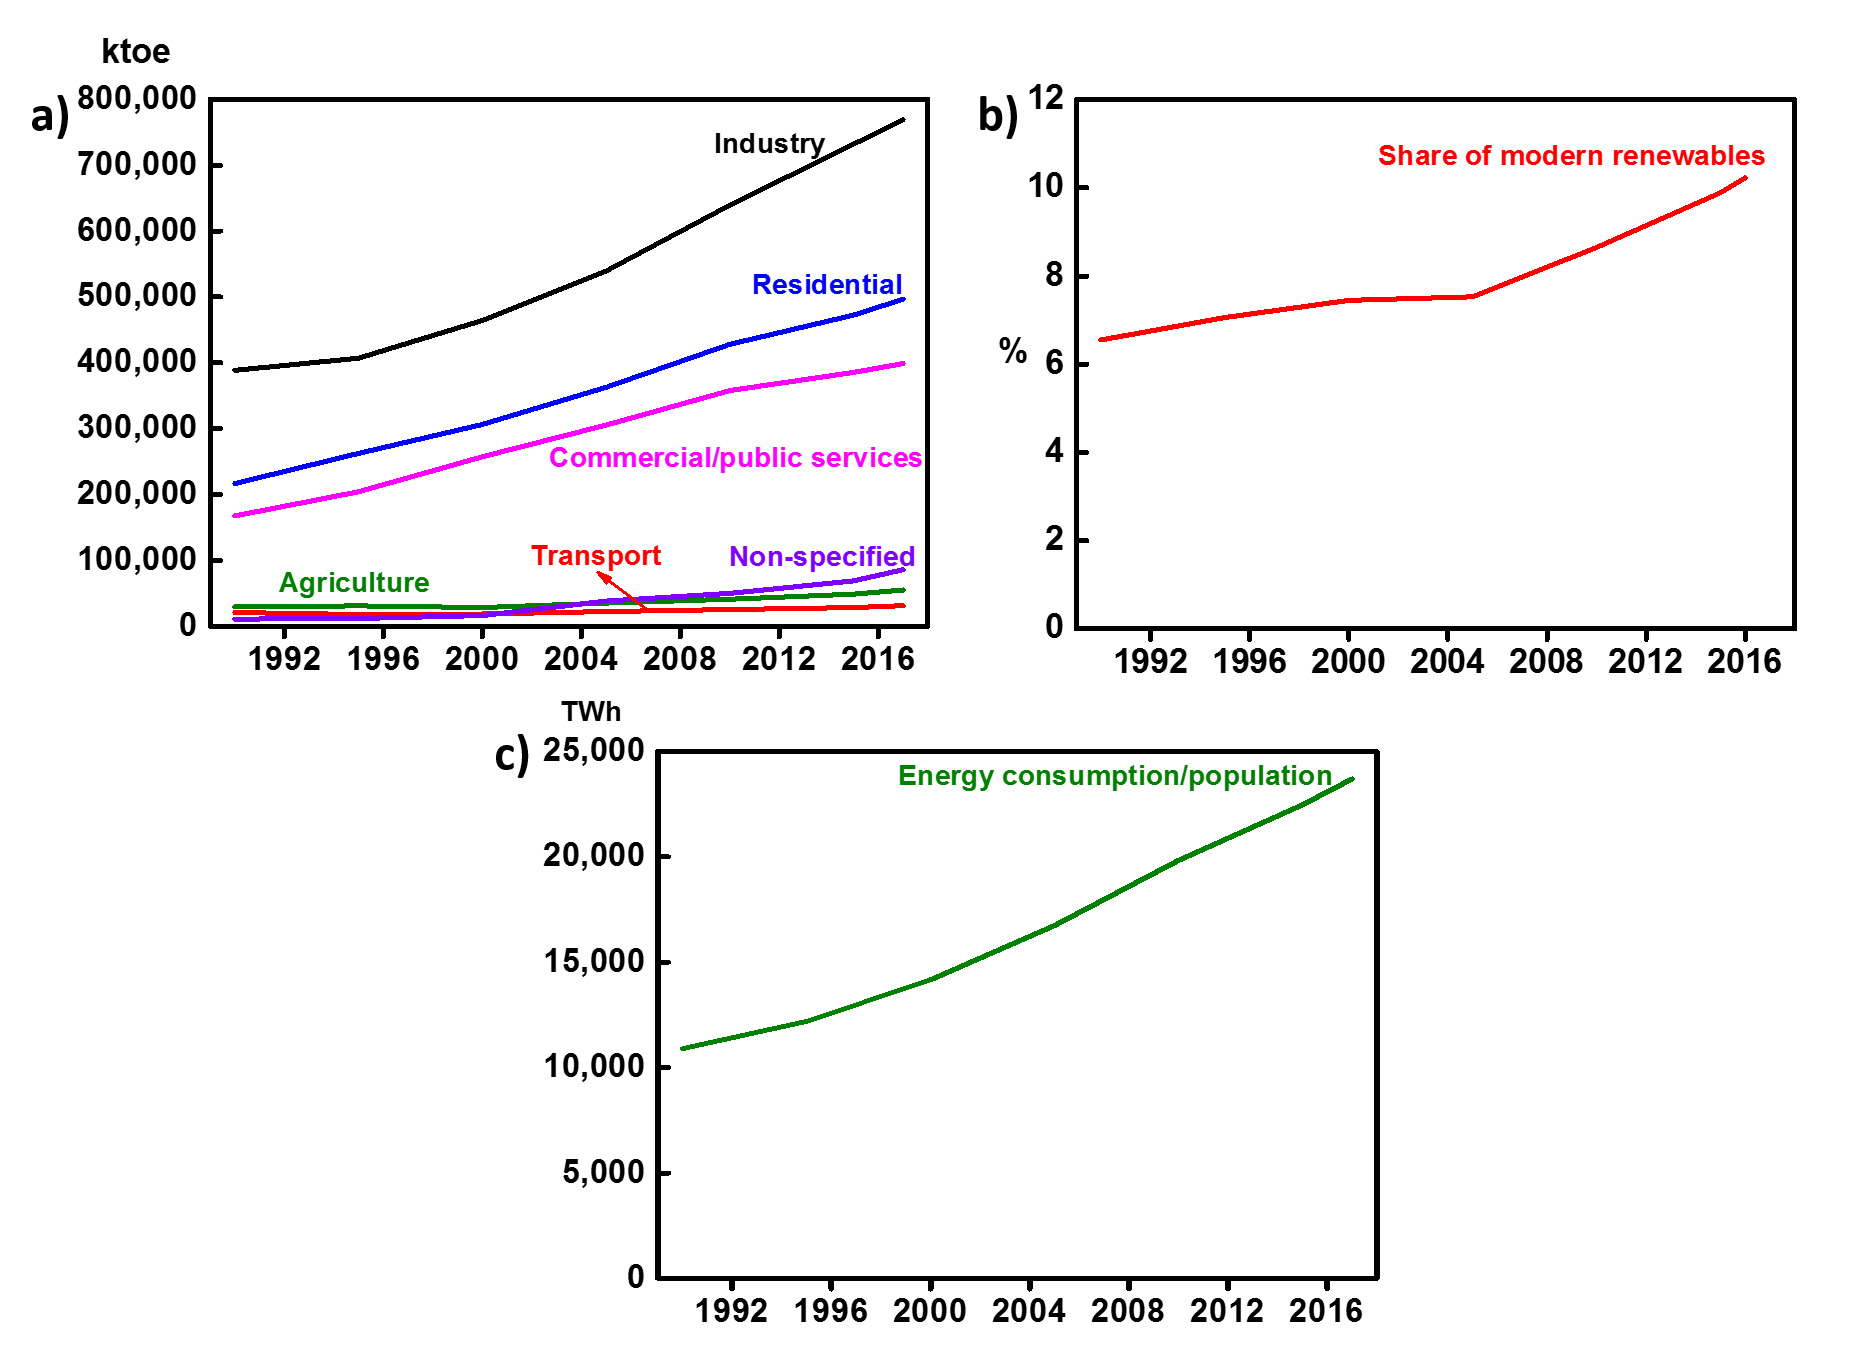
\includegraphics[width=\textwidth]{Figures/chap1fig/IECdata}
\caption{Based on IEA data from the IEA (2018) Monthly Oil Data Service, www.iea.org/statistics. All rights reserved.}
\label{Figures/chap1fig:IECdata}
\end{figure}

\begin{itemize}
\item \textbf{Battery capacity}: Capacity is the amount of charge or energy stored in a battery. Mathematically, it is evaluated by integrating current over time. The fundamental units of battery capacity is coulombs (C), though Amp-hrs (Ah) is more commonly used.  Theoretical capacity (ideal capacity under equilibrium conditions) is calculated with the help of chemical reactions that take place inside the cell. Using Faraday’s constant (F = 96,484.56 C mol$^{-1}$), total available charge in a battery ot its capacity can be determined using equation:

\begin{equation} \label{eq1}
  \text{Capacity(Ah) = } \frac{n \times F \times 1 \text{ hour}}{3600 \text{ sec}}
\end{equation}

\item \textbf{Battery potential}: Voltage is the  most important characteristic of a battery. It is the point usually in the middle of a discharge curve. This is where voltage stays for the longest period during discharge forming a plateau. Various factors help determine a cell's voltage such as electrolyte stability, polarization of the battery and concentrations of the active species. Figure \ref{Figures/chap1fig:CDCforcellvoltage} represents an ideal charge/ discharge curve (CDC). To avoid any permanent damage, a battery should not be discharged below a certain level. This voltage is called the "cut-off voltage". Going beyond a cut-off might lead to certain reactions that decompose the electrolyte (also called side reactions) resulting in an irreversible capacity loss. 

\begin{figure}[tbh!]
\centering
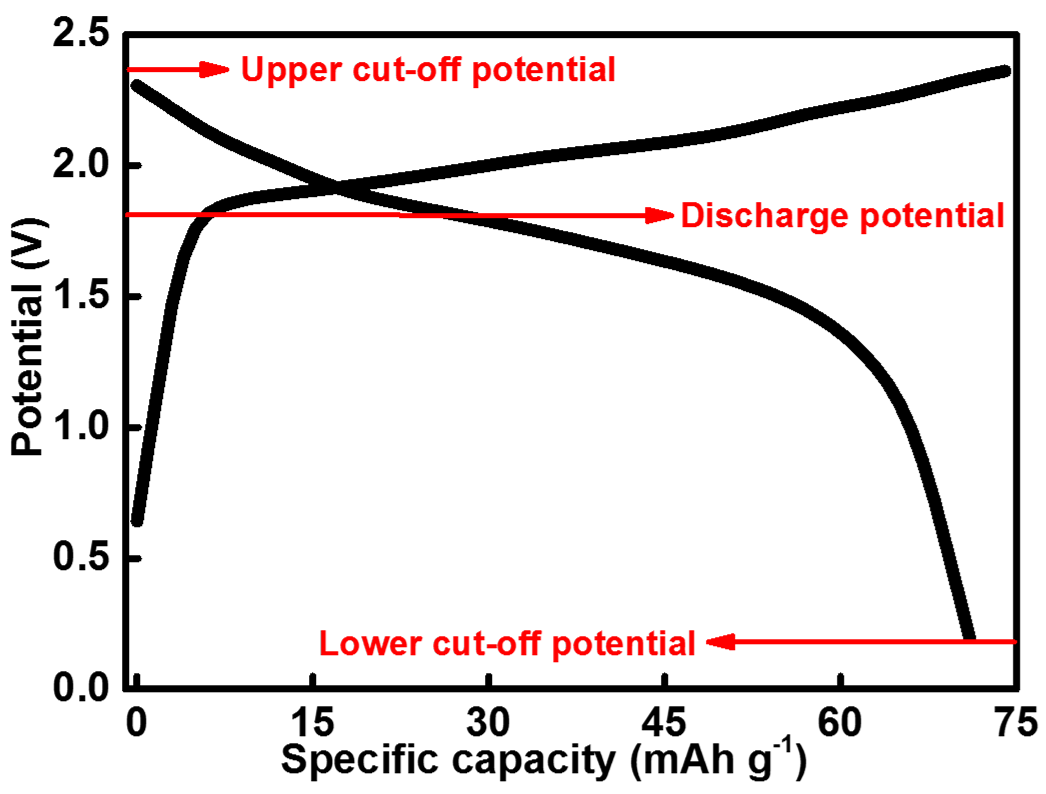
\includegraphics[width=0.75\textwidth]{Figures/chap1fig/CDCforcellvoltage}
\caption{A charge/ discharge curve of an aluminium ion cell using graphite as the cathode and pure aluminium as the anode. The cell was charged and discharged to 2.45 V and 0.2 V respectively.}
\label{Figures/chap1fig:CDCforcellvoltage}
\end{figure}

\item \textbf{Energy density}: The amount of energy stored in a given system per unit mass or volume is called the energy density of a battery. primary function of a battery is to store electrical energy. Heavy batteries are required to move something as large as a car over long distances, therefore they use batteries with high energy density. A simple way to determine the specific energy or energy density of a battery is using Eq.\ref{eq2}:

\begin{equation} \label{eq2}
    \text{Energy density = } \text{Battery capacity (Ah)} \times \text{Battery voltage (V)}
\end{equation}

\item \textbf{Power density}: Power density measures how quickly a battery can deliver energy. Also known as specific power, it's equivalent to the maximum current one can draw from a battery. Units used to describe power density are W kg$^{-1}$ or W m$^{-3}$. The best way to differentiate between energy and power density of a battery is to use an example of a moving car. Energy density determines how 'far' the car will go, whereas power density determines how 'fast' the car will go.

\item \textbf{Coulombic efficiency}: Coulombic efficiency of a battery is the ratio of number of charges that enter during charge to the number that can be extracted from the battery during discharge.  A high coulombic efficiency in excess of 95\% is considered a standard value for commercial battery systems. Any loss in coulombic efficiency can be attributed to some secondary reaction (side reactions) in the battery system. 
\end{itemize}

\textbf{Primary and secondary batteries}: Primary or non-rechargeable batteries produce current immediately when assembled. They have very high energy densities since it is a single-use system. Implanted medical devices, guided missiles, mars rovers and military ordnance use primary batteries. They prove to be an uneconomical energy source since they produce only about 2\% of the power used during their production. Common types of disposable batteries include zinc-carbon and alkaline batteries. 
\textit{Secondary}, or rechargeable batteries, need to be charged before their first use. Since they are  assembled in the discharged state, applying an electric current (during charge) reverses the cell's active materials chemical state. They find extensive use in portable devices as they store energy reversibly. The oldest form of rechargeable battery is the lead-acid battery, which has been used since the 1700's. These batteries find extensive use in automotive, power tools, laptop computers, mobile phones, toys, etc. The most commonly used examples of rechargeable batteries are lithium-ion batteries, nickel-cadmium (NiCad) and nickel metal hydride (NiMH) batteries. 

The charging/discharging rates affect the rated battery capacity. If the battery is being discharged very quickly (high discharge current is applied), then amount of energy that can be extracted from the battery is reduced and its capacity decreases. This is because only a fraction of the total reactants are converted to other forms, and therefore the energy available is reduced. Alternately, if a battery is discharged using low current, more energy can be extracted from the battery and the battery capacity is higher. The temperature of a battery also affects the energy that can be extracted. At a higher temperature, the battery capacity is typically higher than at a lower temperature. However, intentionally elevating battery temperature is not an effective method to increase battery capacity as this also decreases battery lifetime. 
An ideal battery should be low-cost, get charged and discharged indefinitely under high or low current rate, have a long lifetime with high coulombic efficiency (>95\%), and low-self discharge. However, it is difficult to fulfil the above set of requirements. Researchers are building batteries that might achieve these objectives \cite{slater_sodium-ion_2013,jian_carbon_2015,aurbach_prototype_2000,lin_ultrafast_2015-2}. \\

Table\ref{table1} compares a few characteristics of rechargeable batteries that currently exist in market. 

\begin{sidewaystable}
\centering
\caption{Characteristics of commonly used rechargeable batteries.} \label{table1}
\begin{tabular}{ |p{3.5cm}|p{2cm}|p{2cm}|p{2cm}|p{4.5cm}|p{4.5cm}|}
 \hline 
\textbf{Battery type} & \textbf{In market since} & \textbf{Energy density} & \textbf{Nominal voltage (V)} & \textbf{Applications} & \textbf{Limitations}\\ 
\textbf{} & \textbf{} & \textbf{(Wh kg$^{-1}$)} & \textbf{} & \textbf{} & \textbf{}\\ 
\hline
Lead-acid & 1881 & 30-50 & 2.0 & backup power supplies for telephone and computer centres, grid energy storage, uninterrupted power supply (UPS), marine applications- submarines & Environmental hazard, low energy density, risk of thermal runaway, transportation restrictions\\
Nickel-cadmium (Ni-Cad) & 1960 & 40-80 & 1.2 & portable electronics, toys, cordless telephones & Environmental hazard, low energy density, high self-discharge\\
Nickel-metal hydride (Ni-MH) & 1990 & 60-120 & 1.2 & Consumer electronics, electric vehicles, hybrid cars & Expensive, high self-discharge, high maintenance\\
Lithium-ion (\ce{LiCoO2}) & 1991 & 150-190 & 3.6 & Smartphones, laptops, tablets, digital cameras, hybrid vehicles, electric motorcycles, scooters, bicycles, personal transporters & Safety hazard, risk of thermal runaway, transport restrictions, environmental hazard\\
Lithium-ion (\ce{LiMn2O4}) & 1996 & 100-135 & 3.8 & Same as above & Same as above\\
Lithium-ion (\ce{LiPO4}) & 1999 & 90-120 & 3.3 & Same as above & Same as above\\
Lithium-ion (LiNi$_{x}$Co{$_{1-x-y}$}O$_{2}$, LiNMC) & 2008 & 190-210 & 3.6 & Same as above & Same as above\\
\hline
\end{tabular}
\end{sidewaystable}

\newpage

\section{Lithium-ion battery (LIB)}
Standard potential of a redox reaction determines whether a voltage is generated between a redox reaction or not. If the difference between the standard potentials is positive, then the reaction will proceed spontaneously. If the standard potential is negative, a voltage needs to be applied in order for the reaction to proceed, which is precisely what is needed in a battery. Therefore, standard potential is an important parameter to find a suitable battery anode. Lithium has the highest electrochemical potential, which enables it to achieve very high energy and power densities. This is the reason why LIBs are a popular battery-choice for most applications. The most commonly used electrolyte for LIBs is based on lithium hexafluorophosphate (\ce{LiPF6}) and mixture of carbonate solvents. Carbonates such as dimethyl carbonate (DMC), ethyl methyl carbonate (EMC), or diethyl carbonate (DEC), make the electrolyte less viscous and enhance its conductivity. However, they are flammable and show flash points around room temperature (between 16 and 33$^{\circ}$C). In combination with an oxidant and an ignition source, they may catch fire and cause explosions!\\

%LIB is a power pack of choice not only on the Earth, but also in space. In October 2019, a few astronauts on board the International Space Station (ISS) stepped outside their quarters for a spacewalk. Flight engineers Christina Koch and Jessica Meir were assigned the task of manually swapping out two nickel hydrogen (NiH) batteries for one brand new LIB. It was the first ever all-female spacewalk in human history! The battery replacement would not only upgrade the station's electrical system but also extend it's life, at least through 2020's. ISS was launched into orbit in 1998 with 48 NiH batteries. The National Aeronautics and Space Administration (NASA) has started swapping these old batteries, since 2017, with 24 new LIBs  that provide higher energy density and a better power efficiency. Naturally, they had to be careful while handling these heavy batteries (195 kg). LIBs come with a potential risk of thermal runaway, which means an increase in temperature leads to conditions that cause a further increase in temperature, often leading to a destructive result. Inside a pressurised oxygen-rich capsule, the results would have been catastrophic! 

However, future battery demand will place increasing pressure on lithium and cobalt reserves\cite{turchen}. To find a suitable battery system, one needs to examine theoretical specific capacities of different ions that can replace lithium. Metals in the upper left corner of the periodic table, such as sodium (Na), magnesium (Mg), potassium (K) and calcium (Ca) report higher theoretical capacities than the others and can be alternatively used as battery anodes. Table  \ref{table2} shows calculations for a few common metal anodes. 

\begin{table}[tbh!]
\caption{Comparing important parameters of various metal anodes.} \label{table2}
\begin{tabular}{lccccrr}
\hline
 & \textbf{Li} & \textbf{Na} & \textbf{Mg} & \textbf{Al} & \textbf{K} & \textbf{Ca}\\
\hline
Valence electrons & 1 & 1 & 2 & 3 & 1 & 2\\
Specific capacity (mAh g$^{-1}$) & 3862 & 1166 & 2205 & 2980 & 685 & 1340\\
Standard potential (V) & -3.04 & -2.71 & -2.36  & -1.68 & -2.93 & -2.87\\
Abundance (ppm) & 18 & 22700 & 23000 & 82000 & 18400 & 41000\\
\hline  % Please only put a hline at the end of the table
\end{tabular}
\end{table}

High abundance and easy accessibility of aluminium resources enable aluminium-ion batteries (AIBs), together with their electrochemical characteristics and performance, offer the opportunity to become an ideal alternative.

\section{Aluminium-ion battery (AIB)}
The second most promising metal with a relatively high standard oxidation potential is aluminium (Al). AIBs use aluminium metal as anode, which makes it cost-effective, recyclable, and much safer than LIBs. A multivalent ion insertion (intercalation) is feasible, which increases the theoretical energy density of AIBs (Table \ref{table2}. Moreover, the high abundance and easy accessibility of Al resources enable Al-ion batteries to become an ideal candidate for large-scale energy storage system. 

\subsection{Aqueous aluminium-ion batteries (AAIBs)}
The electrolyte is a chemical medium that allows the flow of charge between the cathode and anode. It acts like a catalyst by promoting the movement of ions from the cathode to the anode. The electrolyte of a battery is usually made of soluble salts, acids or other bases in liquid, gelled or dry media, a polymer, or ionic liquids, also known as molten salts. The ions transport current through the electrolyte while the electrons flow in the external circuit generating an electric current. Using water as an electrolyte would reduce the battery costs significantly and increase battery safety. However, these batteries come with their own set of problems. 

\begin{itemize}
    \item the electrochemical plating/stripping of aluminium occurs at a voltage far from the stable potential window of water
    \item aluminium trichloride \ce{AlCl3} is highly acidic and might result in dissolution of active material leading to corrosion of battery parts
    \item a cathode material with a good cycling stability is yet to be discovered
\end{itemize}  

Anatase titanium oxide (\ce{TiO2}) has been investigated as an intercalation electrode for AAIBs. \ce{TiO2} nanostructures have been commonly used as cathode materials in aqueous AIBs. Improving characteristics such as cycle life, efficiency and rate capability would enable these batteries to be used for high power applications. However, limited focus has been given to cycle life, efficiency and rate capability in the recent aqueous Al-ion literature. Cycling data for \ce{TiO2} nanotubes were presented up to cycle 13 by Liu et al \cite{liu_aluminum_2012}.  Recently, a graphene enhanced \ce{TiO2} electrode was shown to produce a capacity between 10 and 25 mAh g$^{-1}$ at a current density of 6.25 A g$^{-1}$. However, only 125 cycles were possible and coulombic efficiency was observed to be very low at approximately 50\%. Similarly, the charge discharge profiles observed for the nanospheres and nanotubes show low coulombic efficiencies of around 80-85\%. The reason for low efficiency of \ce{TiO2} in aqueous AIB electrolyte is yet to be explored, but the possibilities could be oxidation of \ce{Ti3+} due to dissolved \ce{O2} in electrolyte, \ce{H2} gas evolution or an irreversible reduction of \ce{Ti4+} to \ce{Ti2+} while charge.  
Aluminium in aqueous or protic systems forms a passivating oxide film and often corrodes the metal. At standard conditions, it instantaneously forms a very thin (thickness $\sim$2-10 nm), uniform, and continuous amorphous surface layer of \ce{Al2O3} \cite{vargel2004translated}. This oxide film is stable over a pH range of about 4.0-8.6. Although this would be an advantage when using aluminium anode in LIB cathode \cite{myung_electrochemical_2011}, it provides a barrier for solvation of aluminum and transportation of \ce{Al^{3+}}, which poses a big challenge for using Al metal directly as anode.

\subsection{Non-aqueous AIBs}
Chloroaluminates have been known for aluminium electrodeposition since the 1970s and have also been used as electrolytes for rechargeable aluminium batteries. Systems with a general formula MCl-\ce{AlCl3} where \ce{M+} can be a cation like \ce{Na+}, \ce{Li+} or an organic species like pyrrolidinium or immidazolium have been tested as electrolytes for rechargeable AIBs. These melts can be acidic, basic or neutral. In the acidic systems, the dominant species is \ce{Al2Cl7^{-}}, while in a basic system \ce{Cl-} and \ce{AlCl4^{-}} anions coexist whereas in neutral melts, only \ce{AlCl4^{-}} anions exist. Because the standard electrode potential of \ce{Al^{3+}}/Al (-1.68 V) is lower than \ce{H+}/\ce{H2}, the evolution of \ce{H2} occurs due to the reaction between aluminum foil and aqueous acid or alkali solution. Thus, Al cannot be electrochemically striped or deposited in a common aqueous solution. To be compatible with Al anode, the ionic liquid \ce{AlCl3}/[EMIM]Cl with a wider range of electrochemical active window emerges as the typical electrolyte, which provides a mild corrosive effect on the Al surface to activate the Al striping and plating reaction. 

\begin{align*}
        \ce{xAl + 7x\ce{AlCl4-} &<-> 4x\ce{Al2Cl7-} + 3x\ce{e-}}
\end{align*}

\section{Cathodes for secondary batteries}
A usable cathode material should have certain properties- good conductivity, high A number of criteria is considered before selecting a battery electrode. The most important ones being natural. A good battery cathode is stable in the presence of an electrolyte, deliver a good working voltage, a large reversible storage capacity should be obtained at that potential and the electrode should be easy to fabricate. 
Theoretical capacity of a material can be found using :

\begin{equation} \label{eq3}
   C_{t} \text{ = } \frac{n \times F}{3.6 \times M}
\end{equation}\\
where n = number of reactive electrons per formula unit,\\
M = molar weight of the material and\\
F = Faraday constant\\
The formula denotes that a material with low molecular weight and high number of reactive electrons would deliver a high theoretical capacity.

\begin{figure}[h!]
\centering
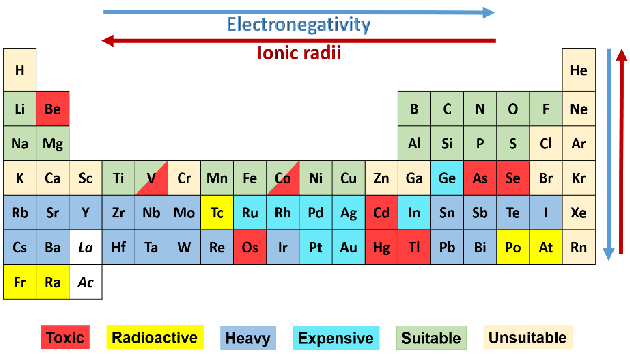
\includegraphics[width=\textwidth]{Figures/chap1fig/pertab}
\caption{The periodic table suggesting elements that can be used as battery materials. However, a few elements from this table have shown good electrochemical performance such as Mo, Sn, Nb and W. Potassium and calcium-ion batteries have also been studied.}
\label{Figures/chap1fig:pertab}
\end{figure}

Figure \ref{Figures/chap1fig:pertab} displays the elements that can be used for designing new cathodes. However, some transition metals such as V or Co, despite their toxicity, have been tried and tested. Transition metals have variable valence states; this increases the number of electrons that can be stored, increasing the battery capacity. The type of bond formed between a metal ion and the ligand plays an important role in determining the electrochemical potential of the material. When the electronegativity difference between the two is high, an ionic bond is formed. A smaller difference results in a covalent bond. Materials with a covalent bonds form poorly packed structures, while ionic bonds form dense structures. A stable structure would enhances the phase stability and electrochemical potential of the material \cite{melot_design_2013}. Furthermore, electrode potential depends on the ionic radius of the material. When an atomic nuclei is loosely bound to its valence electrons, the system needs lower energy for electron transfer , which leads to a lower potential. If more energy is consumed during electron transfer  for materials having a lower ionic radii, the electrochemical potential of the material increases. 

\begin{equation} \label{eq4}
    -\Delta G \text{ = } n \times F \times E
\end{equation}\\
where $\Delta$G = change in internal energy during ion intercalation,\\
n = number of electrons stored per formula unit,\\
F = Faraday constant and\\
E = electrochemical potential of the material. Therefore, the electrochemical potential is affected by interaction between atoms or electrons that change the internal energy. One way to make ionic bonds is to use polyanionic ligands such as phosphates, sulfates and silicates, which are more electronegative. This further enhances the electrochemical potential of a material \cite{melot_design_2013}. For example, \ce{LiCoPO4} displays a higher potential at 4.8 V than \ce{LiCoO2} \cite{masquelier}, which has a potential at 4.0 V. 

\subsection{Cathodes for non-aqueous AIBs}
There are two categories of cathode materials for rechargeable Al batteries. One is the carbon-based materials with high specific surface area. Graphite has been commonly used as a cathode in various battery systems. It has a) a layered structure that enhances the intercalation process, b) good thermal and electrical conductivity and c) a high electrical potential \textit{vs.} \ce{Al}/\ce{Al^{3+}} of 2.1 V. It has a high surface area and good mechanical strength. Many varieties of graphite have since been used in AIBs. Among the carbon-based materials, the highest reported specific capacity (graphene nanoribbons on highly porous 3D-graphene foam) was 148 mAh g$^{-1}$. Fluorinated graphite \cite{rani_fluorinated_2013}, kish graphite flakes \cite{wang_kish_2017-1}, three-dimensional graphitic-foam\cite{wu_3d_2016}, graphene aerogels\cite{huang_graphene_2019} and several other forms have been tested as cathodes for AIBs, which showed specific capacities ranging from 60-250 mAh g$^{-1}$. \ce{AlCl4-}-anions intercalate into the graphitic stacks when the cell is being charged and deintercalate during discharge. Activated carbon, owing to its porous structure, provided a high surface area for absorption of electrolyte ions in super-capacitors \cite{eliad_ion_2001, zhu_carbon-based_2011-2}.
Strong electrostatic nature of trivalent \ce{Al^{3+}} sometimes leads to sluggish kinetics, high over-potentials, and degradation of the host structure. Therefore, to accommodate the highly charged ions, it is essential for the cathode materials to possess weak bond strengths between the host frameworks. The second type with moderate polarity are sulfur, transition metal sulfides, Prussian blue analogues, and some transition metal oxide. These materials have promoted a relatively reversible trivalent reaction. Our unpublished, preliminary density functional theory (DFT) calculations indicated a significant decrease in inter-layer spacing of these materials when \ce{Al^{3+}} cations were assumed to intercalate (owing to the very high charge density of \ce{Al^{3+}}). Therefore, we propose intercalation of \ce{AlCl4-} anions into the layered cathode. XRD, Raman spectroscopy and XPS were used to verify our hypothesis.
Carbon-based materials, molybdenum dichalcogenides, transition metal oxides and a few other materials that would enable transfer of charge-carrying species were tested and the results have been reported in the subsequent chapters.

\section{Research objectives}
The goal of this PhD project is to find new cathodes for rechargeable AIBs that perform better than state-of-the-art. 
\begin{itemize}
    \item Materials that have a layered structure, such as graphite, allow intercalation of charge-carrying species when the cells charge and discharge. We propose that materials with a similar structure, such as molybdenum dichalcogenides, a few transition metal oxides or sulfides, boron nitride (inorganic graphite) would undergo a similar mechanism and deliver a stable performance. 
    
    \item Materials with high surface area such as activated carbon or nano-structured materials, provide a better contact between the cathode and the electrolyte, thus have proven to be good battery materials. They provide a faster and an efficient pathway for electron diffusion, which improves the kinetics of the system and increases the battery's energy density. We tested high surface-area materials such as activated carbon, carbon black, nanostructures of molybdenum dichalcogenides, as cathodes for non-aqueous AIBs to confirm our hypothesis.
    
    \item Once a cathode achieves high capacity (> 60 mAh g$^{-1}$), and a high voltage (> 1.0 V), it is equally important to establish its mechanism. This would help in designing a better cathode. X-ray diffraction studies, Raman spectroscopy, and X-ray photoelectron spectroscopy are a few techniques that have been used to analyse cathode materials. 

\end{itemize}






